\section{Pregunta N$^{\circ}$1\qquad Andre Gilmer Santos Felix}

\begin{frame}
    \begin{definition}[Polinomio de Bernstein]
        Las funciones base de Bernstein son
        \begin{equation*}
            \forall t\in\left[0,1\right]:
            \forall k\in\left\{0,\dotsc,n\right\}:
            B_{k,n}\left(t\right)\coloneqq
            \binom{n}{k}
            t^{k}
            \left(1-t\right)^{n-k}\in\mathbb{P}_{n}.
        \end{equation*}
        Con la convención
        \begin{math}
            B_{-1,n-1}=
            B_{n,n-1}\equiv0
        \end{math}.
    \end{definition}

    \begin{theorem}
        Se cumple
        \begin{math}
            B^{\prime}_{k,n}\left(t\right)=
            n
            \left(
            B_{k-1,n-1}\left(t\right)-
            B_{k,n-1}\left(t\right)
            \right)
        \end{math}.
    \end{theorem}

    \begin{corollary}
        Se cumple
        \begin{math}
            B^{\prime\prime}_{k,n}\left(t\right)=
            n\left(n-1\right)
            \left(
            B_{k-2,n-2}\left(t\right)-
            2B_{k-1,n-2}\left(t\right)+
            B_{k,n-2}\left(t\right)
            \right)
        \end{math}.
    \end{corollary}

    \begin{proof}
        Sea
        \begin{math}
            B_{k,n}\left(t\right)
        \end{math}
        un polinomio de Bernstein.
        Entonces,
        \begin{align*}
            {\left(
                B^{\prime}_{k,n}\left(t\right)
                \right)}^{\prime}
             & =
            \left(
            n
            \left(
            B_{k-1,n-1}\left(t\right)-
            B_{k,n-1}\left(t\right)
            \right)
            \right)^{\prime}. \\
             & =
            n\left(
            \alert{
                B^{\prime}_{k-1,n-1}\left(t\right)
            }    -
            \alert{
                B^{\prime}_{k,n-1}\left(t\right)
            }
            \right).          \\
             & =
            n\left(
            \alert{
                \left(n-1\right)
                \left(
                B_{k-2,n-2}\left(t\right)-
                B_{k-1,n-2}\left(t\right)
                \right)
            }    -
            \alert{
                \left(n-1\right)
                \left(
                B_{k-1,n-2}\left(t\right)-
                B_{k,n-2}\left(t\right)
                \right)
            }
            \right).          \\
             & =
            n\left(n-1\right)
            \left(
            B_{k-2,n-2}\left(t\right)-
            B_{k-1,n-2}\left(t\right)-
            B_{k-1,n-2}\left(t\right)+
            B_{k,n-2}\left(t\right)
            \right).          \\
             & =
            n\left(n-1\right)
            \left(
            B_{k-2,n-2}\left(t\right)-
            2B_{k-1,n-2}\left(t\right)+
            B_{k,n-2}\left(t\right)
            \right).
        \end{align*}
    \end{proof}
\end{frame}

\begin{frame}
    \begin{enumerate}\setcounter{enumi}{0}
        \item

              Calcule la curvatura de la gráfica del polinomio de
              $B_{3,5}\left(t\right)$.
    \end{enumerate}

    \begin{solution}
        Sean los polinomios de Bernstein
        \begin{align*}
            B_{1,3}\left(t\right) & =
            \binom{3}{1}
            t^{1}
            \left(1-t\right)^{3-1}=
            3t{\left(1-t\right)}^{2}.      \\
            B_{2,4}\left(t\right) & =
            \binom{4}{2}
            t^{2}
            \left(1-t\right)^{4-2}=
            6t^{2}{\left(1-t\right)}^{2}.  \\
            B_{3,3}\left(t\right) & =
            \binom{3}{3}
            t^{3}
            \left(1-t\right)^{3-3}=
            t^{3}.                         \\
            B_{3,5}\left(t\right) & =
            \binom{5}{3}
            t^{3}
            \left(1-t\right)^{5-3}=
            10t^{3}{\left(1-t\right)}^{2}. \\
        \end{align*}

        entonces

        \begin{align*}
            B^{\prime}_{3,5}\left(t\right)       & =
            5
            \left[
                B_{2,4}\left(t\right)-
                B_{3,4}\left(t\right)
                \right]=
            5
            \left[
            \binom{4}{2}t^{2}\left(1-t\right)^{4-2}-
            \binom{4}{3}t^{3}\left(1-t\right)^{4-3}
            \right]=                                 \\
            B^{\prime\prime}_{3,5}\left(t\right) & =
            5\left(4\right)
            \left[
                B_{1,3}\left(t\right)-
                B_{3,3}\left(t\right)
                \right]=
            20
            \left[
                B_{2,4}\left(t\right)
                \right].
        \end{align*}

        La curvatura de la gráfica
        \begin{math}
            \left(
            x\left(t\right),
            y\left(t\right)
            \right)=
            \left(
            t,
            B_{3,5}\left(t\right)
            \right)
        \end{math}
        es
        \begin{equation*}
            \kappa\left(t\right)=
            \dfrac{
                y^{\prime\prime}
            }{
                {\left(1+{\left(y^{\prime}\right)}^{2}\right)}^{\frac{3}{2}}
            }=
            \dfrac{
                B^{\prime\prime}_{3,5}\left(t\right)
            }{
                {\left(1+{\left(B^{\prime}_{3,5}\left(t\right)\right)}^{2}\right)}^{\frac{3}{2}}
            }.
        \end{equation*}
    \end{solution}
\end{frame}

\begin{frame}
    \begin{solution}
        \begin{figure}[ht!]
            \centering
            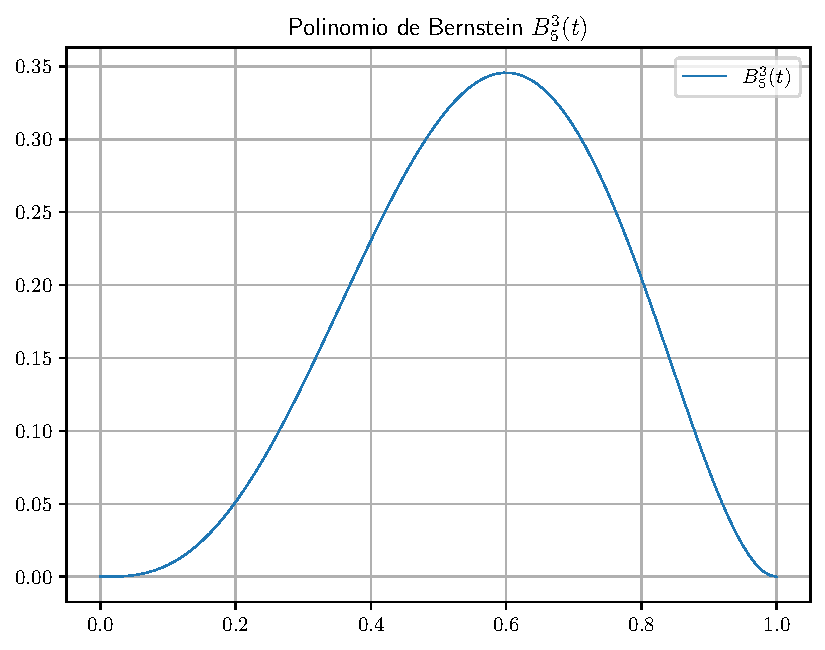
\includegraphics[width=.72\paperwidth]{p1}
        \end{figure}
    \end{solution}
\end{frame}